\documentclass[acmsmall,review,anonymous]{acmart}\settopmatter{printfolios=true,printccs=false,printacmref=false}

\usepackage{tabularx}
\usepackage{amsfonts}
\usepackage{amsmath}
\usepackage{natbib}
\usepackage{graphicx}
\usepackage{tikz}
\usepackage{mathtools}
\usetikzlibrary{chains,fit,shapes,calc}
\usepackage{verbatim}
\usepackage{semantic}
%%\usepackage{DejaVuSansMono}
%%\usepackage{fontspec}
\usepackage[T1]{fontenc}
\usepackage{tabu}
\usepackage{amsthm}
\usepackage{mathptmx}
\usepackage{todonotes}
\usepackage{listings, lstcoq}
\usepackage{ucs}
%%\usepackage[utf8x]{inputenc}
\lstset{language=Coq,
        inputpath=code
       }
\newcommand{\concat}{\ensuremath{+\!\!\!\!+\,}}  

\newtheorem{theorem}{Theorem}[section]
\newtheorem{corollary}{Corollary}[theorem]
\newtheorem{lemma}[theorem]{Lemma}
\newenvironment{proofoutline}
 {\renewcommand\qedsymbol{}\proof[Proof outline]}
 {\endproof}

\begin{document}

\acmJournal{PACMPL}
\acmVolume{1}
\acmNumber{CONF} % CONF = POPL or ICFP or OOPSLA
\acmArticle{1}
\acmYear{2018}
\acmMonth{1}
\acmDOI{} % \acmDOI{10.1145/nnnnnnn.nnnnnnn}
\startPage{1}

%\titlebanner{Preprint}        % These are ignored unless

\title{Verifiably Lazy}
\subtitle{Verified Compilation of Call-by-Need}

\author{George Stelle}
\affiliation{
  \position{Scientist}
  \department{CCS-7}              %% \department is recommended
  \institution{Los Alamos National Laboratory}            %% \institution is required
  \streetaddress{Bikini Atoll Rd., SM 30}
  \city{Los Alamos}
  \state{New Mexico}
  \postcode{87545}
  \country{United States}                    %% \country is recommended
}
\email{stelleg@lanl.gov}          %% \email is recommended

\author{Darko Stefanovic}
\affiliation{
  \position{Professor and Chair}
  \department{Computer Science}              %% \department is recommended
  \institution{University of New Mexico}            %% \institution is required
  \streetaddress{1 University of New Mexico}
  \city{Albuquerque}
  \state{New Mexico}
  \postcode{87131}
  \country{United States}                    %% \country is recommended
}
\email{darko@unm.edu}          %% \email is recommended

\maketitle

\begin{abstract}
We present a verified compiler that preserves call-by-need semantics when
compiling lambda calculus into a simple assembly language. We use a recently
developed abstract machine that implements call-by-need semantics using shared
environments to implement and reason about the compiler. We show that the
abstract machine ensures that the compiled assembly code implements a
call-by-need natural semantics. In addition to the standard proof of correct
results, we prove time complexity is preserved, ensuring that the memoization
of results is preserved. Because call-by-need is an optimization for
call-by-name, we also show the $\beta$ reduction semantics of call-by-name are
preserved.
\end{abstract}

\input{intro}
\input{background}
\section{Cactus Environment Big Step Semantics} \label{sec:cem}

For our call-by-need semantics we turn to the recently developed Cactus
Environment $\mathcal{CE}$ Machine \cite{?}. We break the section in to two
parts. First, we describe environment representation, and the choice we make for
the $\mathcal{CE}$ machine. Next, we describe the big-step semantics of the
machine.

\subsection{Environment Representations}

As mentioned in Section~\ref{sec:back}, environments bind free variables to
closures. There is significant flexibility in how they can be represented. In
this section we review this design space in the context of existing work, both
for call by value and call by need.\footnote{Some work refers to this space as
\emph{closure} representation rather than \emph{environment}
representation~\cite{shao1994space,appel1988optimizing}.  Because the term
part of the closure is simply a code pointer and the interesting design
choices are in the environment, we refer to the topic as environment
representation.}

There are two common approaches to environment representation: \emph{flat}
environments and \emph{shared} environments (also known as linked
environments)~\cite{appel1988optimizing,shao1994space}. A flat environment is
one in which each closure has its own record of the terms its free variables are
bound to. A shared environment is one in which parts of that record can be
shared among multiple closures~\cite{appel1988optimizing,shao1994space}. For
example, consider the following term: $$(\lambda x.(\lambda y.t) (\lambda
z.t_1)) t_2$$ Assuming the term $t$ has both $x$ and $y$ as free variables, we
must evaluate it in the environment binding both $x$ and $y$.  Similarly,
assuming $t_1$ contains both $z$ and $x$ as free variables, we must evaluate it
in an environment containing bindings for both $x$ and $z$. Thus, we can
represent the closures for evaluating $t$ and $t_1$  as $$t[x=t_2[\bullet],
y=c]$$ and $$t_1[x=t_2[\bullet], z=c_1]$$ respectively.  These are examples of
\emph{flat} environments, where each closure comes with its own record of all of
its free variables. Because of the nested scope of the given term, $x$ is bound
to the same closure in the two environments. Thus, we can also create a shared,
linked environment, represented by the following diagram:

\begin{center}
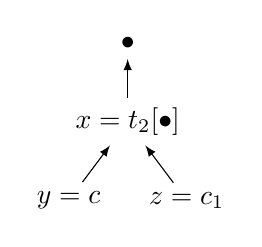
\begin{tikzpicture}[ 
  edge from parent path={(\tikzchildnode\tikzchildanchor) edge [-latex] (\tikzparentnode\tikzparentanchor)},
  level distance=1cm
]
\node (d) {$\bullet$} child{node (a) {$x=t_2[\bullet]$} child{node (b) {$y=c$}} child{node (c)
{$z=c_1$}}};

\end{tikzpicture}
\end{center}

Now each of the environments is represented by a linked list, with the binding
of $x$ shared between them. This is an example of a \emph{shared} environment
~\cite{appel1988optimizing}. This shared, linked structure dates back to the 
first machine for evaluating expressions: Landin's SECD
machine~\cite{landin1964mechanical}.

The primary insight of the $\mathcal{CE}$ machine is that it uses shared
environments to share results between instances of a variable. See \cite{cem}
for more details.

\subsection{Big Step Semantics}

Our big step semantics resemble a hybrid between Curien's calculus of closures
and Ariola et al. call-by-need operational semantics. We use terms with deBruijn
indices and close the the lambda term under a pointer into a shared environment
structure (the Heap).  

The big step semantics can be seen in Figure~\ref{fig:bigstepcem}. The
\texttt{clu} function is a partial function that looks up a closure in the
shared environment. Here we use a direct function, but later this will be
replaced by a relation, as it will clearly take a non-constant number of
instructions to execute. Our abstraction rule is identical to the call-by-name
case, and the application rule evaluates the left hand side, then binds the
argument closure to a fresh location in the heap, which extends the environment
of the function computed on the left hand side. Then if the body with this
extended environment evaluates to a value, then the application as a whole
evaluates to a value.

We define a cactus environment machine state to be well formed if, like Ariola 
et al.'s call-by-name semantics, a closure bound in the heap is closed to the
left.  Effectively, this just means that the head closure, and all closures in
the heap are closed under the heap. One advantage to using deBruijn indices is
that when referring to a fresh heap location, we don't require freshness with
respect to a substitution term, because there is no substitution. This is in
contrast to the operational semantics of Ariola et al \cite{ariola1995call}.

\begin{figure*}
\textbf{Syntax}
\begin{align*}
\tag{Term} t &::= i \; | \; \lambda t \; | \; t \; t  \\
\tag{Variable} i &\in \mathbb{N}  \\
\tag{Closure} c &::= t [l] \\
\tag{Value} v &::= \lambda t [l] \\
\tag{Heap} \mu &::= \epsilon \; | \; \mu [ l \mapsto \rho ] \\
\tag{Environment} \rho &::= \bullet \; | \; c \cdot l \\
\tag{Location} l,f &\in \mathbb{N}  \\
\tag{State} s &::= (c, \mu)
\end{align*}
\textbf{Call-by-Name Semantics}
\begin{align*}
\tag{MVal} \inference {}{(\lambda t, \mu) \rightarrow_M (\lambda t, \mu)}
\end{align*}
\begin{align*}
\tag{MApp} \inference
{(t[l], \mu) \rightarrow_{M} (\lambda t_2[l'], \mu') \quad f \not \in \textnormal{dom}(\mu') \\ 
(t_2[f], \mu'[f \mapsto t_3[l] \cdot l']) \rightarrow_{M} (v, \mu'')}
{(t \; t_3[l], \mu) \rightarrow_{M} (v, \mu'')}  
\end{align*}
\begin{align*}
\tag{MVar} \inference 
{\mu(l, i) = l' \mapsto c \cdot l'' \quad (c, \mu) \rightarrow_M (v, \mu')}
{(i[l],\mu) \rightarrow_M (v,\mu')}
\end{align*}
\textbf{Call-by-Need Semantics}
\begin{align*}
\tag{NVal} \inference{\quad}{(\lambda t, \mu) \rightarrow_N (\lambda t, \mu)}
\end{align*}
\begin{align*}
\tag{NApp} \inference
{(t[l], \mu) \rightarrow_{N} (\lambda t_2[l'], \mu') \quad f \not \in \textnormal{dom}(\mu') \\ 
(t_2[f], \mu'[f \mapsto t_3[l] \cdot l']) \rightarrow_{N} (v, \mu'')}
{(t \; t_3[l], \mu) \rightarrow_{N} (v, \mu'')}  
\end{align*}
\begin{align*}
\tag{NVar} \inference
{\mu(l, i) = l' \mapsto c \cdot l'' \quad (c, \mu) \rightarrow_N (v, \mu')}
{(i[l],\mu) \rightarrow_N (v, \mu'(l' \mapsto v \cdot l''))}
\end{align*}
\caption{Big Step Semantics for $\mathcal{CE}$}
\label{fig:bigstepcem}
\end{figure*}

\subsection{Cost Definitions}

What do we mean when we discuss the time and space complexity for a natural
semantics? Generally, we really care about the the number of instructions that
will be executed in the compiled code, and the maximum amount of memory that
will be necessary, both in the stack and the heap. One advantage to the
simplicity of the compiler for the $\mathcal{CE}$ machine is that we can define
this cost for our natural semantics in a simple way. We do this by defining a 
cost function that operates on the step function directly. This is one of the
useful features of working in a dependently typed proof asistant: we can write
functions that compute values from proof tree. Computing values from proof
objects requires defining our big step relation in the \texttt{Type} universe
instead of the \texttt{Prop} universe, but this isn't a problem.

We define two cost functions: one that computes the time for an evaluation
relation instance, and none that computes the space. Our goal is to define these
such that we can prove that the cost is preserved down through machine code. 

\begin{lstlisting}

\end{lstlisting}

\section{Cactus Environment Small Step Semantics} \label{sec:cesm}

This section describes how we define small step semantics using a stack to track
argument closures from the \texttt{App} rule and update markers from the
\texttt{Id} rule. By defining this intermediate semantics, we ease the proof
burden between the big-step semantics and the assembly machine semantics.   

\subsection{Semantics}

The rules for our small step semantics closely map to the rules of of the big
step semantics. We split the Id and App rules into rules that push and pop off
the stack. The \texttt{Id} rule gets split into the \texttt{Update} and
\texttt{Var'} rules, which take an update marker and replace the closure at that
location with the current value, and push an update marker, respectively. 

One major difference is that we have to drop the reachability requirement here.
Because we have no way to \emph{remember} the reachability ordering without
pushing something onto the stack, we must change our heap to be a monolithic
single heap, and then reason about the existence of a partitioning of the heap
to be equivalent to the big step semantics. This is analagous to a kind of
\emph{erasure} of information about reachability. It does raise questions as to
whether or not there is some way to retain this information for a cheap way to
re-allocate memory, but that is beyond the scope of this work.

Our well formed property for the small step semantics is a bit different, due to
the monolithic heap. We don't actually require any well-formedness property for
the stack, though investigating that possibility would make for interesting
future work. That said, the proof of retention of well-formedeness is much
simpler: there is no inductive step.   

\begin{figure*}
\textbf{Syntax}
\begin{align*}
\tag{State} s &::= \langle c, \sigma, \mu \rangle \\
\tag{Term} t &::= i \; | \; \lambda t \; | \; t \; t  \\
\tag{Variable} i &\in \mathbb{N}  \\
\tag{Closure} c &::= t [l] \\
\tag{Value} v &::= \lambda t[l] \\
\tag{Heap} \mu &::= \epsilon \; | \; \mu [ l \mapsto \rho ] \\
\tag{Environment} \rho &::= \bullet \; | \; c \cdot l \\
\tag{Context} \sigma &::= \square \; | \; \sigma \; c \;  | \; \sigma \; u \\
\tag{Location} l,u,f &\in \mathbb{N}
\end{align*}
\textbf{Semantics}
\begin{align*}
\tag{Upd}
\langle v,  \sigma \; u , \mu \rangle 
  &\rightarrow_{\mathcal{\mathcal{C} \mskip -4mu \mathcal{E}}}
\langle v, \sigma, \mu(u \mapsto v \cdot l) \rangle  
\; \textnormal{where} \; c \cdot l = \mu(u) \\
\tag{Lam}
\langle \lambda t[l], \sigma \; c, \mu \rangle 
  &\rightarrow_{\mathcal{\mathcal{C} \mskip -4mu \mathcal{E}}}
\langle t[f], \sigma, \mu[f \mapsto c \cdot l]\rangle f \not \in \textnormal{dom}(\mu)  \\
\tag{App}
\langle t \; t'[l], \sigma, \mu \rangle
  &\rightarrow_{\mathcal{\mathcal{C} \mskip -4mu \mathcal{E}}}
\langle t[l], \sigma \; t'[l], \mu \rangle \\
\tag{Var}
\langle i[l], \sigma, \mu \rangle
  &\rightarrow_{\mathcal{\mathcal{C} \mskip -4mu \mathcal{E}}}
\langle c[l'], \sigma \; u, \mu \rangle
\; \textnormal{where} \; \mu(l, i) = u \mapsto c \cdot l'
\end{align*}
\caption{Small Step $\mathcal{CE}$ Semantics}
\label{fig:cesm}
\end{figure*}

\subsection{Relation to Big Step $\mathcal{CE}$ Semantics}

We prove that the cesm implements the big-step semantics and the reflexive
transitive closure of the small-step semantics. The relation itself is generally
uninteresting; the heap structure is essentially the same so we require equality
of the heap and concatenation of the big step heaps, and we require nothing of
the stack. Furthermore, the terms and closures are equivalent. Really, the only
goal of this proof is to show that the stack preserves the computation
structure.  

\begin{lstlisting}
Lemma bigstep_smallstep : ∀ c h v h' s, 
  big.step (big.st c h) (big.st v h') → 
  refl_trans_clos small.step (small.st c s h) (small.st v s h')
\end{lstlisting}

\begin{proofoutline}
By induction on the bigstep relation.
\end{proofoutline}

Note that the relation is defined on the reflexive transitive closure of the
small-step relation \emph{for all stacks}. We use the fact that this implies
that the same relation will hold for the empty stack, which is the initial and
final state of the small-step machine, as desired.


\section{Instruction Machine} \label{sec:mach}

In this section we describe the instruction machine syntax and semantics, and
how the relation with the stack machine from the previous section works. We can
then write down the full relation to the natural semantics of the source by
composing this relation with the big-step to small-step relation. We thus end
up with our final proof, namely that the call-by-need semantics are preserved
by the machine semantics. 

\subsection{Instruction Assembly}

Our instruction syntax is described in Section~\ref{sec:intro}. Unlike the
relation between the big step and small step semantics, the relation between
the smallstep semantics and the instruction machine semantics requires an 
assembly step. The assembler compiles lambda terms with deBruijn indices into
instructions. It is in fact the only program transformation in this compiler, 
which is a testament the ease of compilation of the $\mathcal{CE}$ machine.

We give the full assembly function in Figure~\ref{fig:assemble}. 

\begin{figure}
\begin{lstlisting}
Fixpoint var_inst (i : nat) : BasicBlock := match i with
  | 0 => push EP ;
         push (RC 0) ;
         mov (EP%0) R1 ;
         mov (EP%1) EP ;
         jump None R1
  | S i => mov EP (EP%2) ;
           var_inst i
  end.

Fixpoint assemble (t : tm) (k : nat) : Program := match t with  
  | var v => [var_inst v]
  | app m n => let ms := assemble m (k+1) in
               let nk := k + 1 + length ms in
                 push EP ;
                 push (RC nk) ;
                 jump None (RC (k+1)) :: 
                 ms ++ 
                 assemble n nk
  | lam b => pop R1 ;
             jump (Some (RW (WR R1), (k+1))) (RC (k+2)) ::
             (*Update*)
             pop R1 ;  
             mov (RC k) (R1%0) ;
             mov EP (R1%1) ;
             jump None (RC k) ::
             (*Take*)
             new 3 R2 ;
             mov R1 (R2%0);
             pop (R2%1) ;
             mov EP (R2%2) ;
             mov R2 EP ;
             jump None (k+3) ::
             assemble b (k+3)
  end. 
\end{lstlisting}
\caption{Assembler in Coq}
\end{figure}

For variables, the code compiles a basic block that follows the shared
environment pointer the appropriate number of times, followed by pushing an
update marker pointing to the closure in the heap that will be updated. For
the application, we push the argument closure onto the stack then continue
into the left hand side. This push-enter style compiler is the simplest to 
reason about, though investigating eval-apply could make for interesting future
work. Finally, abstractions are compiled into three basic blocks, the first checks
if the top of the stack is an update marker or a instruction pointer and branches
appropriately, while the second performs the update by replacing the closure 
at the update location with the current closure, and the third binds the 
argument closure to a new heap location. Note that our new location requires three
machine words: the instruction pointer, environment pointer pair that makes 
up the closure, as well as the shared environment pointer pointing to the 
environment that was extended with said closure. 

\subsection{Machine Semantics}

The machine semantics are fairly straightf given the instructions and
machine state. We omit the full semantics, though they are available in the
source Coq files.

Some of the less obvious semantics: a closure is represented as two machine
words, or \texttt{nat}s in our case. The first is an instruction pointer. The
second is an environment pointer pointing into the heap. Our current closure is
defined by our instruction pointer and environment pointer registers. 

In general, the machine semantics are fairly predictable given the instructions 
available. The \texttt{pop} instruction pops a machine word off of the stack and
into the write operand, while the \texttt{push} reads the read operand and pushes
it onto the stack. While we have implemented the stack as a list of words, it 
would be straightforward future work to lower this further to be implemented as
an in-memory array. Our \texttt{new} instruction returns an unused chunk of
memory of the given size. Note that as with the small step $\mathcal{CE}$ semantics,
in the future the semantics should be updated to be able to re-use dead memory
locations, something which we currently don't manage. 

We implement our program as a finite map from machine pointers to basic blocks. 
Because we use the null pointer as a marker for updates on the stack, we start
our basic block indices at 1. As with the stack, it would make for
straightforward future work to replace the instruction pointer so that the
instructions and basic blocks were represented in memory directly. 

On the stack, we differentiate between update markers and argument closures by
using a zero in place of an instruction pointer, therefore disallowing a zero
instruction pointer, in agreement with modern conventions. We can then check for
zero on the top of the stack using the optional first argument to our jump
instruction. If the argument operand is zero, then we jump to the given
constant location, otherwise we jump the fallback second argument. 

\subsection{Relation with Small Step $\mathcal{CE}$ Semantics}

We define our relation on the basic blocks created by the compiler. We relate
the machine and small step states in fairly simple ways. The deBruijn terms of
the small step semantics are all replaced with instruction pointers, and we
require that the mapping preserves a program equivalence. This relation relies
on the fact that each subterm corresponds with a subprogram starting at the given
instruction pointer.
 
Once we have a notion of program equivalence, we can define a notion of
environment equivalence. This is defined by induction on the environment
structure, requiring that every term reachable by that $\mathcal{CE}$
environment is equivalent to the corresponding instruction pointer in the 
instruction machine for a given program. Combined with program equivalence, we
can define a closure equivalence relation to relate the instruction machine closures
with the $\mathcal{CE}$ machine closures. Once we have that relation, we can
define a relation to relate the complete instruction machine states with the
$\mathcal{CE}$ machine state. We then show that this relation holds for the
initial states for each, and that it holds by induction on the step relation
of the $\mathcal{CE}$ machine.

\begin{figure}
\begin{lstlisting}

\end{lstlisting}
\caption{}
\end{figure}

For execution of instructions, we relate each rule in the small step semantics
to a basic block of code. Note that we've artificially increased the number of
instructions in this case and could trivially show that a sound optimization
is removing all of the unconditional \texttt{jmp} instructions to the next
basic block.  

In the same way substitution is often modeled as a single step, when
implementing the lookup in the machine semantics we must convert our
\texttt{clu} to a an inductive lookup executed by machine instructions. Of
course, this takes a number of instructions proportional to the size of the
deBruijn index. Our program equivalence relation ensures the number of steps
the \texttt{clu} lookup takes is equivalent to the number of indirections
taken by the generated code.

Our heap relation is fairly straightforward. Each cell of the $\mathcal{CE}$
semantics corresponds with three machine words: for the closure there will be an
instruction pointer and an environment pointer, and then one machine words for
the environment continuation. A cell is equivalent to one of these triplets iff
the instruction pointer points to a basic block that is equivalent to the term,
and the environment pointers are equivalent modulo heap location isomorphism.

Note that we do require that the \texttt{new} instruction returns a block of
machine words. This is in contrast to flat representations, where it needs to
return blocks of variables sizes. This is also a situation in which the
simplicity of the $\mathcal{CE}$ machine is very valuable: because of this
constant sized closures, we don't need to worry about cases in which the
value closure that we update a heap location with has more free variables, and
therefore requires more space, leading to the need for indirections as in the
STG machine \cite{STG}.



\input{applications}
\input{discussion}
\section{Conclusion} \label{sec:conclusion}

We have shown how to build a verified compiler that verifies time and space
requirements in addition to the usual correctness properties. We have used this
technique to build a verified compiler of call-by-need, proving that the
memoization of results is implemented correctly. This is the first
machine-checked proof that an optimization is \emph{preserved through
compilation} that we are aware of. 

Typed functional language programmers have long leaned on the important property
that their programs "can't go wrong". Historically this property has always
included an important asterisk: "unless it runs out of time or memory". Without
tools to reason formally about time and memory usage this asterisk is impossible
to confront. We have shown how one can reason formally about properties like
stack size and heap size, in a way that is preserved to machine code, enabling
programmers to finally manage this wart.




% We recommend abbrvnat bibliography style.
\bibliographystyle{abbrvnat}
\bibliography{annotated}

\end{document}
